\documentclass{article}

\usepackage[utf8]{inputenc}
\usepackage[T1]{fontenc}
\usepackage{microtype}
\usepackage{amsmath}
\usepackage{url}

%\usepackage[superscript,biblabel,nomove]{cite}
\usepackage[super,square]{natbib}

\usepackage{newspaper}

\date{NOVEMBER 29, 1982}
\currentvolume{1}
\currentissue{1}

%% [LianTze] The newspaper package also provides
%% these commands to set various metadata:

%% The banner headline on the first page
%%   (The colon after s: is to get a more
%%   modern majuscule s in this font instead of
%%   the medieval tall s. For anyone interested
%%   in the history:
%%  http://medievalwriting.50megs.com/scripts/letters/historys.htm)
\SetPaperName{%
  \fontencoding{T1}\fontfamily{phv}\fontsize{36}{0}\bfseries
  Physics Yesterday%
}
%% The name used in the running header after
%% the first page
\SetHeaderName{Physics Yesterday}

%% and also...
\SetPaperLocation{New York}
\SetPaperSlogan{``Yesterday's physics, delivered today''}
\SetPaperPrice{}


% [LianTze] times (the package not the font) is rather outdated now; use newtx (see later)
% \usepackage{times}
\usepackage{graphicx}
\usepackage{multicol}
\graphicspath{images}
\usepackage{caption}

\usepackage{picinpar}
%uasage of picinpar:
%\begin{window}[1,l,\includegraphics{},caption]xxxxx\end{window}


%% [LianTze] Contains some modifications
\usepackage{newspaper-mod}
%%... so now you can redefine the headline and byline style if you want to.
%% These can be issued just before any
%% byline or headline in the paper, to
%% individually style each article
%%
% \renewcommand{\headlinestyle}{\itshape\Large\lsstyle}
% \renewcommand{\bylinestyle}{\bfseries\Large\raggedright}

\newcommand{\q}[1]{\vspace{10pt}
\textbf{#1}}

%Needed to make the figure env work with multicol
\newenvironment{Figure}
  {\par\medskip\noindent\minipage{\linewidth}}
  {\endminipage\par\medskip}

%%%%%%%%%  Front matter   %%%%%%%%%%

\begin{document}
\maketitle

\begin{multicols}{2}

\byline{The Asymmetric Life of Dr. Wu}{Alice Pleasance Liddell}

\textit{Chien-Shiung Wu, hailed as the first lady of physics, retired last year with numerous accolades to her name. She made extraordinary contributions to her field, such as proving that parity is not conserved. She was the American Physical Society’s first female president\cite{N12} and won the inaugural Wolf Prize\cite{N11}. Today we interview her to hear her reflections on her life and research.}
\vspace{10pt}

\begin{Figure}
 \centering
 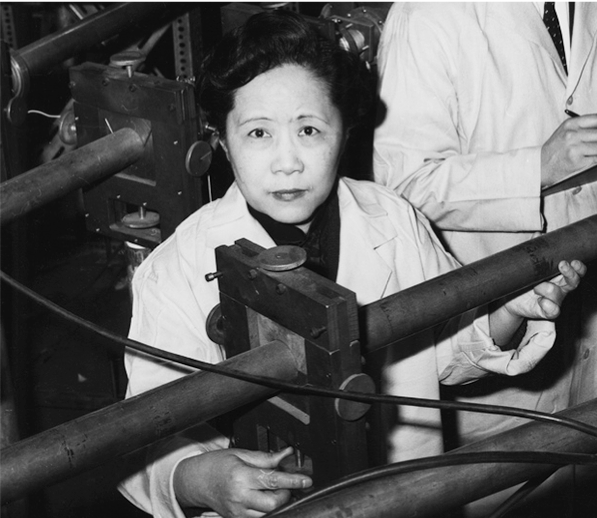
\includegraphics[width=0.9\linewidth]{{./images/wu-columbia}.png}
 \captionof{figure}{\textit{\footnotesize Chien-Shiung Wu in 1963 at Columbia University}}
\end{Figure}


%\begin{window}[10,r,\includegraphics[width=2in]{{"./images/wu-columbia"}.png},
%\textit{\footnotesize Chien-Shiung Wu in 1963 at Columbia University}
%]
\textbf{Welcome, Chien-Shiung Wu, it’s a privilege to have you here today. You’ve been retired for a year now, but throughout your life you’ve made some remarkable discoveries and become a role model for women all over the world. What motivated you to pursue physics? Did you have role models of your own at an early age? }

Thank you. When I was a student, I came across a biography of Madame Curie, the great chemist and physicist who became the first woman to win a Nobel Prize\cite{L1}. Curie’s intellectual curiosity and perseverance in a field dominated by men was particularly inspiring to me as a girl, and it ignited a lifelong passion. As a teenager I spent all my free time teaching myself physics from textbooks borrowed from friends and would often study late at night. I fell in love with physics. Neither friends, nor family, could pull me away from my work – \textit{I have always felt that in physics, and probably in other endeavors too, you must have total commitment. It is not just a job; it is a way of life} \cite{L2}. I knew, however, that I would face many challenges, not only as a woman but as a Chinese American. My father encouraged me and gave me the confidence to succeed. He founded my elementary school, which was one of the first to admit girls. It was still very uncommon for girls to attend school then, but he strongly believed that girls should receive an education. I remember him always telling me to ignore the obstacles and keep walking forward – so I did\cite{L3}.
%\end{window}

\q{Indeed, you’ve earned the nickname ``the Chinese Madame Curie\cite{L1}''. What a prestigious title! That must be something, given you were so inspired by her.}


\textit{People think that calling me the Chinese Madame Curie is an endorsement and honour, but I do not quite feel that way}\cite{L5}. It disappoints me that I must be compared to a western female physicist for my work to be valued. My father instilled in me a pride in Chinese culture that I will always harbour.

\q{Of course, you should be credited in your own right. The most important name is your own; Chien-Shiung means “a strong hero” in Chinese, which is a wonderful tribute to your trailblazing role in the scientific community \cite{L6}. You have become a hero to women everywhere. What would you say to them?}

Women should pursue careers in science, and I am glad that more are entering science fields. \textit{It’s shameful that there are so few women in science. This is the fault of men}\cite{N1}. We are just as powerful as men, and we’re just as intelligent. We’re capable of making fantastic discoveries and contributing to science whilst remaining eternally feminine. Look at Madame Curie! Lise Meitner! Such fantastic women. \textit{Never before have so few contributed so much under such trying circumstances} \cite{L6}. Women should know they are just as capable as men.

\q{You graduated in 1934 at the top of your class with a Physics degree from Nanjing University \cite{L7}. Congratulations, that is quite an achievement. How did you continue to pursue your career in science after your degree?}

Thank you. Yes, I graduated during a time when physics was becoming one of the liveliest and exciting research areas in the world, with breakthroughs like Albert Einstein’s theory of relativity making the field revolutionary. China had no graduate programme for aspiring physicists and so I moved to the United States in August 1936. I was accepted for a PhD position at the University of Michigan, but I didn’t believe that women shouldn’t be allowed to use the front entrance to the university… so I decided to carry out my research at the University of Berkeley instead. That’s where I met Professor Ernest Lawrence. I was lucky to have him as an academic supervisor as his invention of the cyclotron made him a Nobel Prize winner, and I carried out part of my thesis in his radiation laboratory \cite{L5}.

\q{That’s remarkable! I can’t imagine how proud your family were of you back in China. Did you manage to stay in contact with them?}

Sadly not. A year into my PhD I received news that Japan had invaded China. I didn’t hear from my parents for eight years.

\q{That must have been incredibly difficult for you. What was life like for you in the US during the war?}

I struggled, particularly as a Chinese immigrant in the US. I was living a double life – one where I was a physicist doing exciting research. And another where I was an immigrant separated from my family, living in a country with rising anti-Asian sentiments \cite{N2}.

\q{How did the rising prejudice affect your career and life?}

I had many opportunities cut off to me and struggled to find a research position. I have always preferred to wear my qipao (my traditional Chinese dress), even underneath my lab coat \cite{N3}. So this has further marked me out as different.

\q{Despite the constant worries I’m sure you had about your family and friends in a war-torn China, you still thrived at Berkeley. You even met your husband there, right?}

Yes, I met Chia-Liu at Berkeley; he was a fellow student. After I’d graduated with my PhD we got married in May 1942 and moved to the East coast \cite{Nbroken}. Neither of our families could attend the wedding because of the Second World War fighting in the Pacific. I remember how much we feared for them at the time.

\q{I’m sorry, Dr. Wu. When were you able to see your family again?}

I received a letter from them after the war, once communication with China was restored. I planned to visit them but never got the chance because the Chinese Civil War then started, and my father told me not to return to Communist China. By the time I came home in 1973, my parents, brother and uncle had died. Their tombs had been destroyed. I didn't get the chance to say goodbye.

\q{You worked on the world-changing Manhattan Project during the war. How did that happen?}

In 1941 I had started to work on nuclei decay and fission. I was invited to an interview at Columbia, where the research was classified. The interviewers were so secretive, and they didn’t talk about the research details. But even with this, I realised what they were researching! I spent two days interviewing in different rooms, and saw the equations scribbled on the blackboards in all the rooms, so I pieced it all together. They laughed when I told them I had figured it out and offered me the position \cite{N4}.

\q{What can you tell us about the Manhattan Project?}

I worked on enriching uranium so that it could be used for the atom bomb. We have a lot of uranium-238, but this is very stable and is not fissionable. Instead, we wanted more uranium-235 to be used in nuclear fission. Uranium-235 is sparse in nature, so I worked on obtaining it from uranium-238. I also helped to improve the accuracy of Geiger counters \cite{Nbroken}.

\q{That’s fascinating. How did you feel about your work being used to create nuclear weapons?}

I do regret that the nuclear weapons created were used on Hiroshima and Nagasaki \cite{N7}. It was a great tragedy, and the devastation was vast and will be felt for decades. It saddens me. I really hope that the bomb was a one off, and that it will not happen again. \textit{Surely people aren’t so stupid and self-destructive? No. I have confidence in humankind} \cite{N7}.

\q{Hopefully, it doesn't happen again - I’m sure we can all agree with that. Clearly you have worked on many pivotal experiments in your lifetime. Which one would you say that you were most excited about?}

I love them all! But if I had to choose, I was extremely excited to work on the parity experiment. I didn’t go on vacation to China just to work on it. Chia-Liu and I had planned to return to China after having left twenty years earlier. Our passages were already booked. But then I had the sudden realization that I had to do the experiment immediately. So, I asked Chia-Liu to let me stay and go without me \cite{N14}.

\q{I keep hearing about this experiment on parity violation, but everywhere I turn, I can’t seem to find a good explanation! All this talk about mirrors, parallel universes, symmetries… How does it really work?}

Let’s start simple – you mentioned mirrors. Imagine you’re standing in front of one: now, hold out your right hand, pointing your index finger towards your reflection, and keeping your thumb and middle finger perpendicular to your index. What do you see?

\begin{Figure}
 \centering
 \includegraphics[width=\linewidth]{{"images/parity-diagram"}.png}
 \captionof{figure}{\textit{\footnotesize Polar vectors flip when mirrored, but axial vectors stay the same}}
\end{Figure}



\q{My index finger is pointing in the opposite direction, but my other fingers aren’t… Hmm…}

Exactly - there’s something different about your mirror image – something that isn’t just a rotation, which would have moved all your fingers equally, but which really changes the relationship between the different directions in space. This is where the trick comes in. Let’s go back to the mirror: but this time, instead of pointing towards it, try curling your fingers in a circle parallel to the glass.

\q{Yes, let’s see… Oh. OH! It doesn’t change direction!}

Yes! You see, there are two different “fingers” in our universe: straight fingers, which will get flipped inside mirrors, and curled fingers, which still turn in the same direction. We call these \textit{polar vectors}, or \textit{axial vectors} if they curl around. The mirroring operation is a \textit{parity transformation}, and a \textit{parity symmetry} is anything that doesn’t change under such a transformation.

\q{This is beginning to make sense. So, the next step is looking around for things that break this symmetry?}

Indeed! You’d be surprised, for a long time no one in the physics world dared question this symmetry being universal \cite{N7}. But even just by thinking about this difference between vectors, you can deduce that this isn’t necessarily true. I showed that this isn’t a symmetry for a certain type of interaction – the so-called weak interactions – but there’s a good chance we’ll find more symmetry breaking. Maybe the strong force might be hiding a few asymmetric secrets...

\q{How did you show the weak interaction breaks parity symmetry? I imagine you couldn’t just bring your experimental setup to a flipped universe by crawling through a broken mirror!}

That certainly would have made things more straightforward! However, this is where all the talk of axial versus normal vectors comes in. The weak force is primarily encountered in radioactive decay processes, where it can cause neutrons to decay, releasing an electron. Like most subatomic particles, the neutron has a spin – you can think of it as some rotational motion that the particle goes through, even if that isn’t entirely accurate. What is accurate, though, is thinking of this spin as an axial vector!

\q{So, all you’d need is a normal vector to compare it to, and their relationship won't be symmetric under parity!}

Yes, I needed a polar vector – in this case, the average direction in which the electrons would be emitted. Let’s do a small thought experiment – assume for a moment this decay is the same as in its mirror image. Now, imagine we look at this process several times, and notice that electrons tend to be emitted opposite the direction of spin. What happens if we were to bring this whole setup to a mirror world, and repeat the experiment?

\q{Well, if the direction in which electrons are emitted is a vector, then it will flip – but the direction in which the neutron spins won’t, right?}

Exactly! If we were to look at the neutron from the direction of outgoing electrons, we’d see the particle spin in the opposite direction. However, that would break our assumption that the system does not change in the mirror world. So, you see, if there is any preference at all in the direction in which electrons are emitted, then there is no choice but to break this mirror symmetry \cite{J3}. Such a deceptively simple idea, but truly a revolutionary consequence!



\begin{Figure}
 \centering
 \includegraphics[width=\linewidth]{{"images/decay-diagram"}.png}
 \captionof{figure}{\textit{\footnotesize When we look at the decay in a mirror, we see that any anisotropy in the emission of electrons (green) will flip with respect to the spin direction}}
\end{Figure}

%\begin{window}[2,r,\includegraphics[width=2in]{{"./images/wu-setup"}.png},
%\textit{\footnotesize Diagram of the setup \cite{C3} \vspace{5pt}}
%]
\q{Surely it wasn’t that simple in practice. What was the experiment like?}

We wanted to investigate the parity conservation of beta decay, so the first thing we needed was a beta decay source. We used Cobalt-60, which decays as $^{60}_{27}\text{Co} \rightarrow ^{60}_{27}\text{Ni} + e^{-} + \nu _{e} +2\gamma$ \cite{C1}.
We then aligned the spins of the nucleons using strong magnetic fields, while keeping everything as cold as we could: barely above 1K \cite{C2}! All of this took place inside a specific apparatus, with two pairs of detectors at right angles, to measure both the gamma rays and the electrons.

\begin{Figure}
 \centering
 \includegraphics[width=0.75\linewidth]{{"./images/wu-setup"}.png}
 \captionof{figure}{\textit{\footnotesize  Diagram of the experimental setup \cite{C3}}}
\end{Figure}
\vspace{10pt}
\q{Why the cold temperatures?}

Cobalt atoms vibrate, and this can disturb the alignment during the polarisation step. To avoid this, we freeze the atoms by exposing them to an extremely cold environment!
Using the detectors, we were then able to measure the emission of both electrons and gamma rays in two perpendicular directions and, as the setup heated up, could compare the values as the neutron alignment was broken.
%\end{window}

\begin{Figure}
 \centering
 \includegraphics[width=\linewidth]{{"./images/wu-results"}.png}
 \captionof{figure}{\textit{\footnotesize  Experimental data from Wu’s experiment – the anisotropy in emission of electrons (bottom) perfectly matches that in the emission of gamma rays (top) \cite{C3}}}
\end{Figure}

%\begin{window}[1,r,\includegraphics[width=2in]{{"./images/wu-results"}.png},
%\textit{\footnotesize Experimental data from Wu’s experiment – the anisotropy in emission of electrons (bottom) %perfectly matches that in the emission of gamma rays (top) \cite{C3} \vspace{5pt}}]
\q{I get measuring electrons, but why gamma rays? They’re not directly produced by the weak force.}

You can think of this as a calibration test. We know that gamma rays couple with spin, so we’d expect to see some level of anisotropy \cite{J3}.

This means we now have a way to directly measure how well aligned the nucleons are, and correlate any anisotropy in the electron emissions directly to the weak process, eliminating the chance of external effects influencing our data.
The gamma ray anisotropy that we measured was approximately 0.6, meaning that 60\% of the rays were emitted in one direction, and the remaining 40\% in the other. More importantly, we also measured an anisotropy in the electron emission, which matched the exact plot of the gamma anisotropy\cite{C3}!
%\end{window}

\q{There’s still one question I have – we don’t see electromagnetism breaking parity, so why does the weak force act different?}

That’s not an easy thing to explain. That said, some recent work (begun by Feynman and Gell-Mann\cite{J2}, and then extended by Yang and Mills) is giving us some insight into how the weak force works, and even how it unifies with electromagnetism. In QM, we represent particles as wave-functions – but this begins to break down when we add many particles to the mix. It turns out that we can think of particles not as single entities, but as quantised excitations of fields, which evolve based on some scalar function of the field itself. We call this function the \textit{lagrangian}, and it’s the most important component of any theory – it describes the characteristics of particles, and how different fields interact with each other. Any properties the lagrangian has, such as some symmetry, will correspond to behaviours of particles or interactions\cite{J1}.

\q{So, the lagrangian tells the fields how to move, and the fields tell the lagrangian what value to be?}

Yes, that’s a very good way of putting it. So, what would happen if there was some field whose lagrangian depended on some combination of axial and polar vectors?

\q{The lagrangian wouldn’t be the same under parity, and therefore whatever it’s describing must break that same symmetry!}

Exactly! The big breakthrough was finding that function, and making sure it corresponded to the weak interaction. What Yang and Mills have done is postulate a viable lagrangian describing the interaction of two fermions, and forced it to be rotationally symmetric everywhere. However, the only way to do this is to introduce an additional field – something called a \textit{gauge field}. This field won’t affect how the Lagrangian evolves, but allows us to remove some derivative terms that would otherwise break that symmetry.

This gauge field must be a field of vectors, as it must transform properly under rotations. We label it \textbf{W}, and the particles it describes are the W bosons. If we try to find how this new field modifies the lagrangian, we encounter a term that looks like the sum of a polar vector (derivatives of \textbf{W} itself), and an axial vector (which is formed by a cross-product of different covariant components of \textbf{W})\cite{J1}. However, this new contribution makes the lagrangian lose its mirror symmetry, as a difference between these two types of vectors will definitely not be invariant under parity!

\q{As many have said, this caused a revolution in theoretical physics! The Nobel prize in 1957 was awarded to Chen Ning Yang and Tsung-Dao Lee for disproving parity conservation\cite{N8}. You were not included despite your obviously central part in the experiment.}

\textit{Although I did not do research just for the prize, it still hurts me a lot that my work was overlooked for certain reasons.} I still reveled in the absolute excitement, the pure visceral joy that comes from expanding the human understanding and unlocking another secret of our universe. That was worth it. That was why I researched.

\vspace{10pt}
\q{What reasons do you think your work was overlooked?}

I feel that my gender is a large part of the reason and it does sadden me\cite{N15}. I hope someday we will all be treated as equals. \textit{I wonder if the tiny atoms and nuclei, or the mathematical symbols, or the DNA molecules have any preference for either masculine or feminine treatment}\cite{N9}...

\q{Certainly, and you are a huge advocate for promoting women in science. Thank you for joining us, we’ve gained some insight into the complex field of physics and your fascinating life as a pioneer. Do you have any last words for readers?}

I hope I've shown that science can be learned and explored by everyone – all it takes is a bit of creativity, and ideas that were once thought of as fundamental may prove to be nothing more than a wall of smoke. \textit{There are moments of exhilaration and ecstasy! A glimpse of this wonder can be the reward of a lifetime} \cite{N10}.

\closearticle



\end{multicols}

\newpage
\bibliographystyle{plain}
\bibliography{liberty,naiyira,jacopo,chirag}

\end{document}
